\capitulocapa[48]{images/cap-2.png}{Quando useState deixa de ser suficiente?}
\label{chap:limites-use-state}

\refstepcounter{section}
\addcontentsline{toc}{section}{\protect\numberline{\thesection}Funcionou até o pedido seguinte}
\sectionmark{Funcionou até o pedido seguinte}

\begin{center}
  \makebox[\textwidth][c]{%
    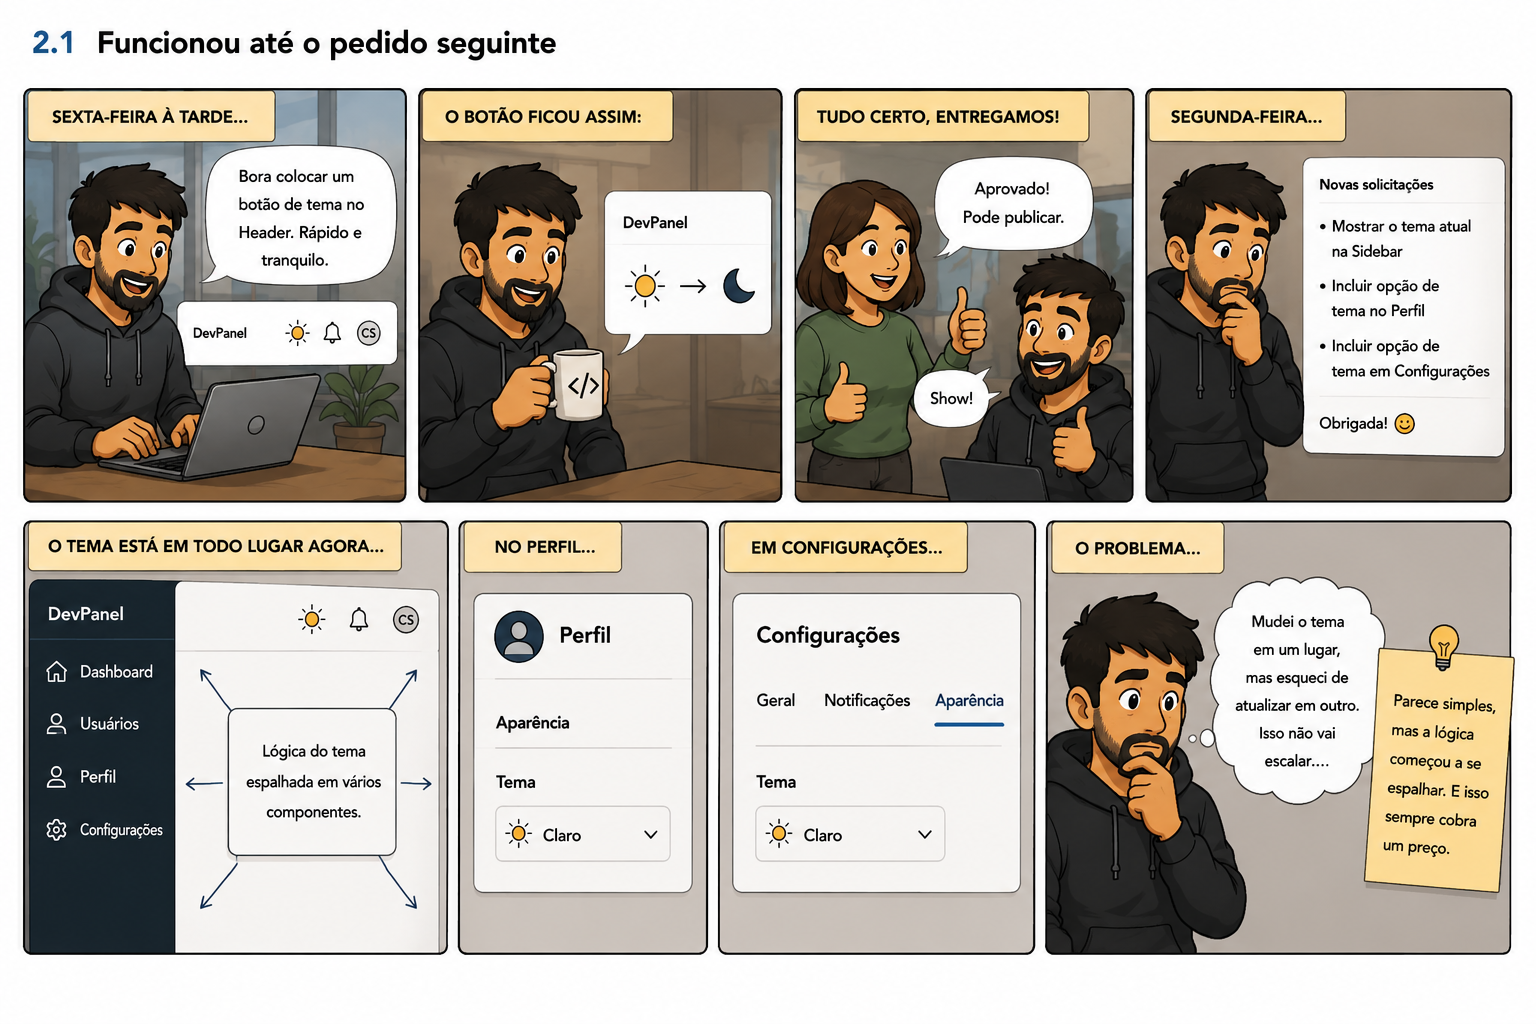
\includegraphics[width=1.16\textwidth]{images/2-1-funcionou-ate-pedido-seguinte.png}%
  }
\end{center}

Esse é um dos momentos mais comuns numa aplicação React. O \codigo{useState}
não parou de funcionar. O requisito é que mudou de tamanho.

Enquanto apenas o Header precisava saber o tema, estado local era uma decisão
razoável. Quando várias regiões passaram a depender da mesma informação, o
alcance do estado deixou de combinar com o alcance da funcionalidade.

\section{O problema: o estado está preso no Header}

A primeira versão do controle é pequena:

\begin{lstlisting}[caption={O tema pertence apenas ao Header nesta primeira versão.},label={lst:header-theme-local}]
import { useState } from 'react'

type Theme = 'light' | 'dark'

export function Header() {
  const [theme, setTheme] = useState<Theme>('light')

  function toggleTheme() {
    setTheme((current) => (current === 'light' ? 'dark' : 'light'))
  }

  return (
    <header className={`header header--${theme}`}>
      <span>Tema: {theme === 'light' ? 'claro' : 'escuro'}</span>
      <button type="button" onClick={toggleTheme}>
        Alternar tema
      </button>
    </header>
  )
}
\end{lstlisting}

Dentro desse limite, não há nada errado. O Header guarda o valor, exibe o valor
e oferece a ação que o modifica. A implementação é fácil de encontrar e de
entender.

O problema aparece quando o componente de Perfil precisa mostrar algo como:

\begin{lstlisting}
export function ProfilePage() {
  return <p>Tema atual: {/* como obter o tema aqui? */}</p>
}
\end{lstlisting}

\codigo{ProfilePage} não é filho de \codigo{Header}. Um componente não consegue
entrar em outro componente e buscar seu estado local. Essa limitação é
intencional: cada renderização possui sua própria memória, associada à posição
daquele componente na árvore.

\section{Como normalmente tentamos resolver}

Quando a demanda chega com prazo curto, algumas saídas parecem menores do que
reorganizar os componentes.

\subsection{Criar outro estado}

Podemos colocar outro \codigo{useState} no Perfil:

\begin{lstlisting}
export function ProfilePage() {
  const [theme, setTheme] = useState<Theme>('light')
  // ...
}
\end{lstlisting}

Agora existem dois temas. Alterar um não altera o outro. O Header pode dizer
``escuro'' enquanto o Perfil diz ``claro''. Não compartilhamos estado; criamos
duas fontes de verdade com o mesmo nome.

\subsection{Ler a interface}

Outra tentativa é inspecionar uma classe no elemento raiz ou ler um atributo do
DOM. Isso troca uma dependência explícita por uma dependência escondida. O
Perfil passa a conhecer detalhes da implementação visual do Header, e o React
continua sem uma fonte de verdade comum para renderizar os dois.

\subsection{Usar armazenamento do navegador como mensageiro}

Também é possível gravar o tema no \codigo{localStorage} e fazer cada tela
consultá-lo. Persistência, porém, não é comunicação reativa. Uma escrita não
garante que todos os componentes renderizem novamente. Além disso, introduzimos
uma preocupação nova --- lembrar o valor depois de fechar o navegador --- antes
de resolver o compartilhamento dentro da tela atual.

\begin{decisao}
Quando dois lugares precisam representar a mesma informação, duplicar o valor
não torna o estado compartilhado. Torna a sincronização responsabilidade do
time. Procure primeiro uma única fonte de verdade.
\end{decisao}

\section{O sinal mais importante: quem precisa saber?}

Antes de escolher Context ou instalar uma biblioteca, vale listar os
consumidores reais:

\begin{itemize}
  \item o Header mostra o botão e o tema atual;
  \item a Sidebar ajusta sua aparência;
  \item o Perfil mostra a preferência selecionada;
  \item Configurações permite alterar a preferência.
\end{itemize}

Essa lista muda a pergunta. Em vez de ``como faço o Perfil acessar o estado do
Header?'', perguntamos ``qual lugar é responsável por um valor usado por todas
essas regiões?''.

O Header deixou de ser uma boa resposta. Ele é apenas um dos consumidores.
Colocar a fonte de verdade dentro dele dá a um detalhe da interface a
responsabilidade por uma preferência da aplicação.

\ilustracaopendente{ch02-mapa-consumidores-tema}{Árvore do DevPanel destacando Header, Sidebar, Perfil e Configurações como consumidores do mesmo tema.}

Essa análise é mais valiosa que contar quantos componentes existem. Dois irmãos
podem justificar estado compartilhado. Dez componentes dentro de um mesmo
formulário podem continuar bem atendidos por estado local. O que importa é a
fronteira de responsabilidade e o ciclo de vida necessário.

\section{Limitações de manter tudo local}

\subsection{Passagem de propriedades}

Para compartilhar um valor usando apenas React, movemos o estado para um
ancestral comum e passamos dados e ações por propriedades. Essa é uma solução
válida e será implementada no próximo capítulo.

O custo aparece quando componentes intermediários recebem propriedades que não
usam, apenas para entregá-las a alguém mais abaixo. A árvore passa a influenciar
a assinatura de vários componentes.

\subsection{Acoplamento à estrutura}

Se movermos o Perfil para outra região, talvez seja necessário refazer o caminho
das propriedades. A funcionalidade passa a depender não apenas de quem precisa
do valor, mas de como os componentes estão encaixados naquele momento.

\subsection{Mudanças espalhadas}

Adicionar uma nova preferência pode exigir mudanças no ancestral, no Header, no
Layout e na página consumidora. Nenhum arquivo é especialmente complexo, mas a
alteração atravessa vários arquivos que não tomam parte na decisão.

\subsection{Ciclo de vida inadequado}

Se o Header for removido numa rota específica, seu estado também desaparece.
Uma preferência da aplicação não deveria depender da presença de um cabeçalho.
O lugar escolhido para o estado determina por quanto tempo ele existe.

\section{Uma solução melhor começa pelo lugar}

Ainda não precisamos escolher a ferramenta final. Primeiro, precisamos aceitar
que o tema não pertence mais ao Header.

Uma solução melhor deve oferecer:

\begin{enumerate}
  \item uma única fonte de verdade para o tema;
  \item leitura pelos componentes que realmente usam o valor;
  \item uma ação compartilhada para alterar a preferência;
  \item ciclo de vida compatível com todo o DevPanel;
  \item dependências visíveis no código.
\end{enumerate}

O React já oferece uma primeira técnica: elevar o estado para o ancestral comum
mais próximo. Se a árvore for curta, essa pode ser toda a arquitetura necessária.
Se o caminho atravessar muitas camadas, sentiremos o custo antes de avaliar
Context ou Zustand.

Essa ordem importa. Uma ferramenta global não deve ser a reação automática ao
primeiro estado usado por dois componentes. Primeiro identificamos a fonte de
verdade; depois escolhemos o mecanismo de distribuição.

\section{Implementação: deixe o limite visível}

Neste capítulo, manteremos a primeira versão local. Mas vamos separar o controle
visual da regra de alternância, deixando explícito o contrato que precisará sair
do Header:

\begin{lstlisting}[caption={O botão recebe o valor e a ação de que precisa.}]
type ThemeToggleProps = {
  theme: Theme
  onToggle: () => void
}

export function ThemeToggle({ theme, onToggle }: ThemeToggleProps) {
  const nextTheme = theme === 'light' ? 'escuro' : 'claro'

  return (
    <button type="button" onClick={onToggle}>
      Usar tema {nextTheme}
    </button>
  )
}
\end{lstlisting}

O Header continua dono do estado, mas o botão não. Ele recebe o valor atual e
uma ação. Isso não resolve o Perfil; apenas separa duas responsabilidades e
torna o próximo movimento mais seguro.

\begin{lstlisting}[caption={A fonte de verdade ainda está local.}]
export function Header() {
  const [theme, setTheme] = useState<Theme>('light')

  function toggleTheme() {
    setTheme((current) => (current === 'light' ? 'dark' : 'light'))
  }

  return <ThemeToggle theme={theme} onToggle={toggleTheme} />
}
\end{lstlisting}

Quando elevarmos o estado, \codigo{ThemeToggle} não precisará mudar. Somente o
componente que fornece \codigo{theme} e \codigo{onToggle} será diferente.

\section{Entendendo as decisões}

\subsection{Um tipo com dois valores válidos}

\begin{lstlisting}
type Theme = 'light' | 'dark'
\end{lstlisting}

O tipo impede estados vagos como uma string vazia ou \codigo{'blue'}. Se o tema
só possui duas opções, o contrato deve dizer isso.

\subsection{Atualização baseada no valor anterior}

\begin{lstlisting}
setTheme((current) => (current === 'light' ? 'dark' : 'light'))
\end{lstlisting}

O próximo tema depende do tema atual. Por isso usamos a forma funcional da
atualização. A função recebe o valor mais recente conhecido pelo React e devolve
o próximo.

\subsection{Ação em vez de setter exposto}

O botão recebe \codigo{onToggle}, não \codigo{setTheme}. Seu trabalho é pedir
uma alternância, não conhecer como o estado é armazenado. Essa diferença ficará
importante quando a fonte de verdade mudar de lugar.

\section{Exercício: faça o desconforto aparecer}

\begin{tarefa}
Crie uma tela de Perfil e exiba nela o tema atual. Por enquanto, mantenha o
\codigo{useState} dentro do Header. Você pode passar propriedades, criar
callbacks ou reorganizar os componentes, mas não use Context, Zustand nem
armazenamento do navegador.
\end{tarefa}

Depois da tentativa, registre:

\begin{enumerate}
  \item por quais componentes o tema precisou passar;
  \item quais componentes receberam dados que não utilizam;
  \item onde ficou a ação de alternar o tema;
  \item qual componente parece ser o ancestral comum correto;
  \item em que ponto a solução começou a parecer frágil.
\end{enumerate}

\espacoresposta{9}

O objetivo não é encontrar um truque. É sentir na prática que o requisito não
combina mais com o lugar onde o estado nasceu. No próximo capítulo, moveremos a
fonte de verdade e acompanharemos o caminho das propriedades pela árvore.

\begin{resumo}
\begin{itemize}
  \item \codigo{useState} não deixa de funcionar; o alcance do requisito é que
    pode deixar de ser local.
  \item Repetir o mesmo estado em vários componentes cria fontes de verdade
    independentes.
  \item Persistência não substitui comunicação reativa entre componentes.
  \item A lista de consumidores ajuda a encontrar a responsabilidade correta.
  \item Primeiro decidimos onde o estado deve viver; depois escolhemos como
    distribuí-lo.
\end{itemize}
\end{resumo}

Ainda não chegamos ao Zustand. Agora, porém, existe um problema concreto que
justifica continuar a jornada.
